\chapter{Opis struktury projektu}
\section{Technologie wykorzystane w projekcie}

\textbf{Interfejs użytkownika}

Do budowy interfejsu graficznego zastosowałem technologię WPF (Windows Presentation Foundation) wraz z językiem 
znaczników XAML. WPF został wybrany ze względu na integrację z platformą .NET, bogaty zestaw wbudowanych 
kontrolek oraz możliwość tworzenia nowoczesnych interfejsów bez konieczności stosowania zewnętrznych bibliotek 
graficznych. XAML umożliwia deklaratywne definiowanie interfejsu w sposób czytelny i całkowicie oddzielony od 
logiki aplikacji.

\vspace{10pt}

\textbf{Dostęp do danych}

Do komunikacji z bazą danych wykorzystałem ADO.NET ze sterownikiem Microsoft.Data.SqlClient w wersji 7.0.1. ADO.NET 
został wybrany ze względu na pełną kontrolę nad wykonywanymi zapytaniami SQL. 

\vspace{10pt}

\textbf{Baza danych}

Jako system zarządzania bazą danych wybrałem Microsoft SQL Server 2025 ze względu na to, że używaliśmy go na labach. 
SQL Server oferuje obsługę zaawansowanych typów danych wykorzystanych w projekcie, 
takich jak TIME, DATE czy DECIMAL, a także zapewnia wydajne mechanizmy wymuszania integralności danych poprzez 
klucze obce i ograniczenia CHECK.

\vspace{10pt}

\textbf{Język programowania i platforma}

Aplikacja została napisana w języku C\# na platformie .NET 10.0. Platforma .NET 10.0 zapewnia 
nowoczesne możliwości języka oraz wysoką wydajność.

\vspace{10pt}

\textbf{Narzędzia deweloperskie}

Projekt był rozwijany przy użyciu Visual Studio 2026 Insiders, zintegrowanego środowiska programistycznego 
firmy Microsoft, oferującego zaawansowane narzędzia do debugowania
oraz zarządzania pakietami NuGet. Do zarządzania wersjami kodu użyłem systemu Git z repozytorium na 
platformie GitHub.

\section{Baza danych}
\subsection{Konfiguracja bazy danych (SQL Server)}

W projekcie wykorzystano relacyjną bazę danych Microsoft SQL Server. 
Do jej zarządzania zaleca się użycie narzędzia SQL Server Management 
Studio (SSMS), przewodnik do instalacji (SSMS) można znaleźć pod adresem: 
\url{https://learn.microsoft.com/en-us/ssms/install/install}. W trakcie instalacji 
SQL Server należy wybrać tryb uwierzytelniania Windows 
Authentication. Do poprawnego działania aplikacji należy:

\begin{enumerate}
    \item Otworzyć SQL Server Management Studio i połączyć się z serwerem przy użyciu Windows Authentication.
    \item W panelu Object Explorer kliknąć prawym przyciskiem myszy na Databases i wybrać opcję New Database, a następnie nadać jej nazwę \textbf{klinika\_weterynaryjna}.
    \item Kliknąć prawym przyciskiem myszy na nowo utworzoną bazę danych i wybrać opcję New Query.
    \item Wkleić zawartość pliku \textbf{schema.sql} do edytora zapytań, a następnie kliknąć przycisk Execute (F5).
    \item Po poprawnym wykonaniu skryptu baza danych będzie zawierać wszystkie tabele oraz dane początkowe niezbędne do działania aplikacji.
\end{enumerate}

\subsection{Połączenie z bazą danych w Visual Studio}

Aby aplikacja mogła nawiązać połączenie z bazą danych 
SQL Server, wymagana jest odpowiednia konfiguracja połączenia w 
kodzie źródłowym. Za połączenie z bazą danych odpowiada klasa Database.

\lstinputlisting[caption=Klasa Database, label=dbconnection]{src/DBConnection.cs}

\subsection{Konfiguracja środowiska Visual Studio}

Do uruchomienia projektu w Visual Studio 2026 Insiders 
potrzebujesz platformy .NET 10.0 lub nowszej, działającego serwera 
SQL Server 2025 oraz sterownika Microsoft.Data.SqlClient 
(instalowanego przez NuGet). Konfiguracja projektu obejmuje wybór 
odpowiedniej wersji .NET oraz listę 
poprawnie załadowanych zależności NuGet.

\begin{figure}[H]
\centering
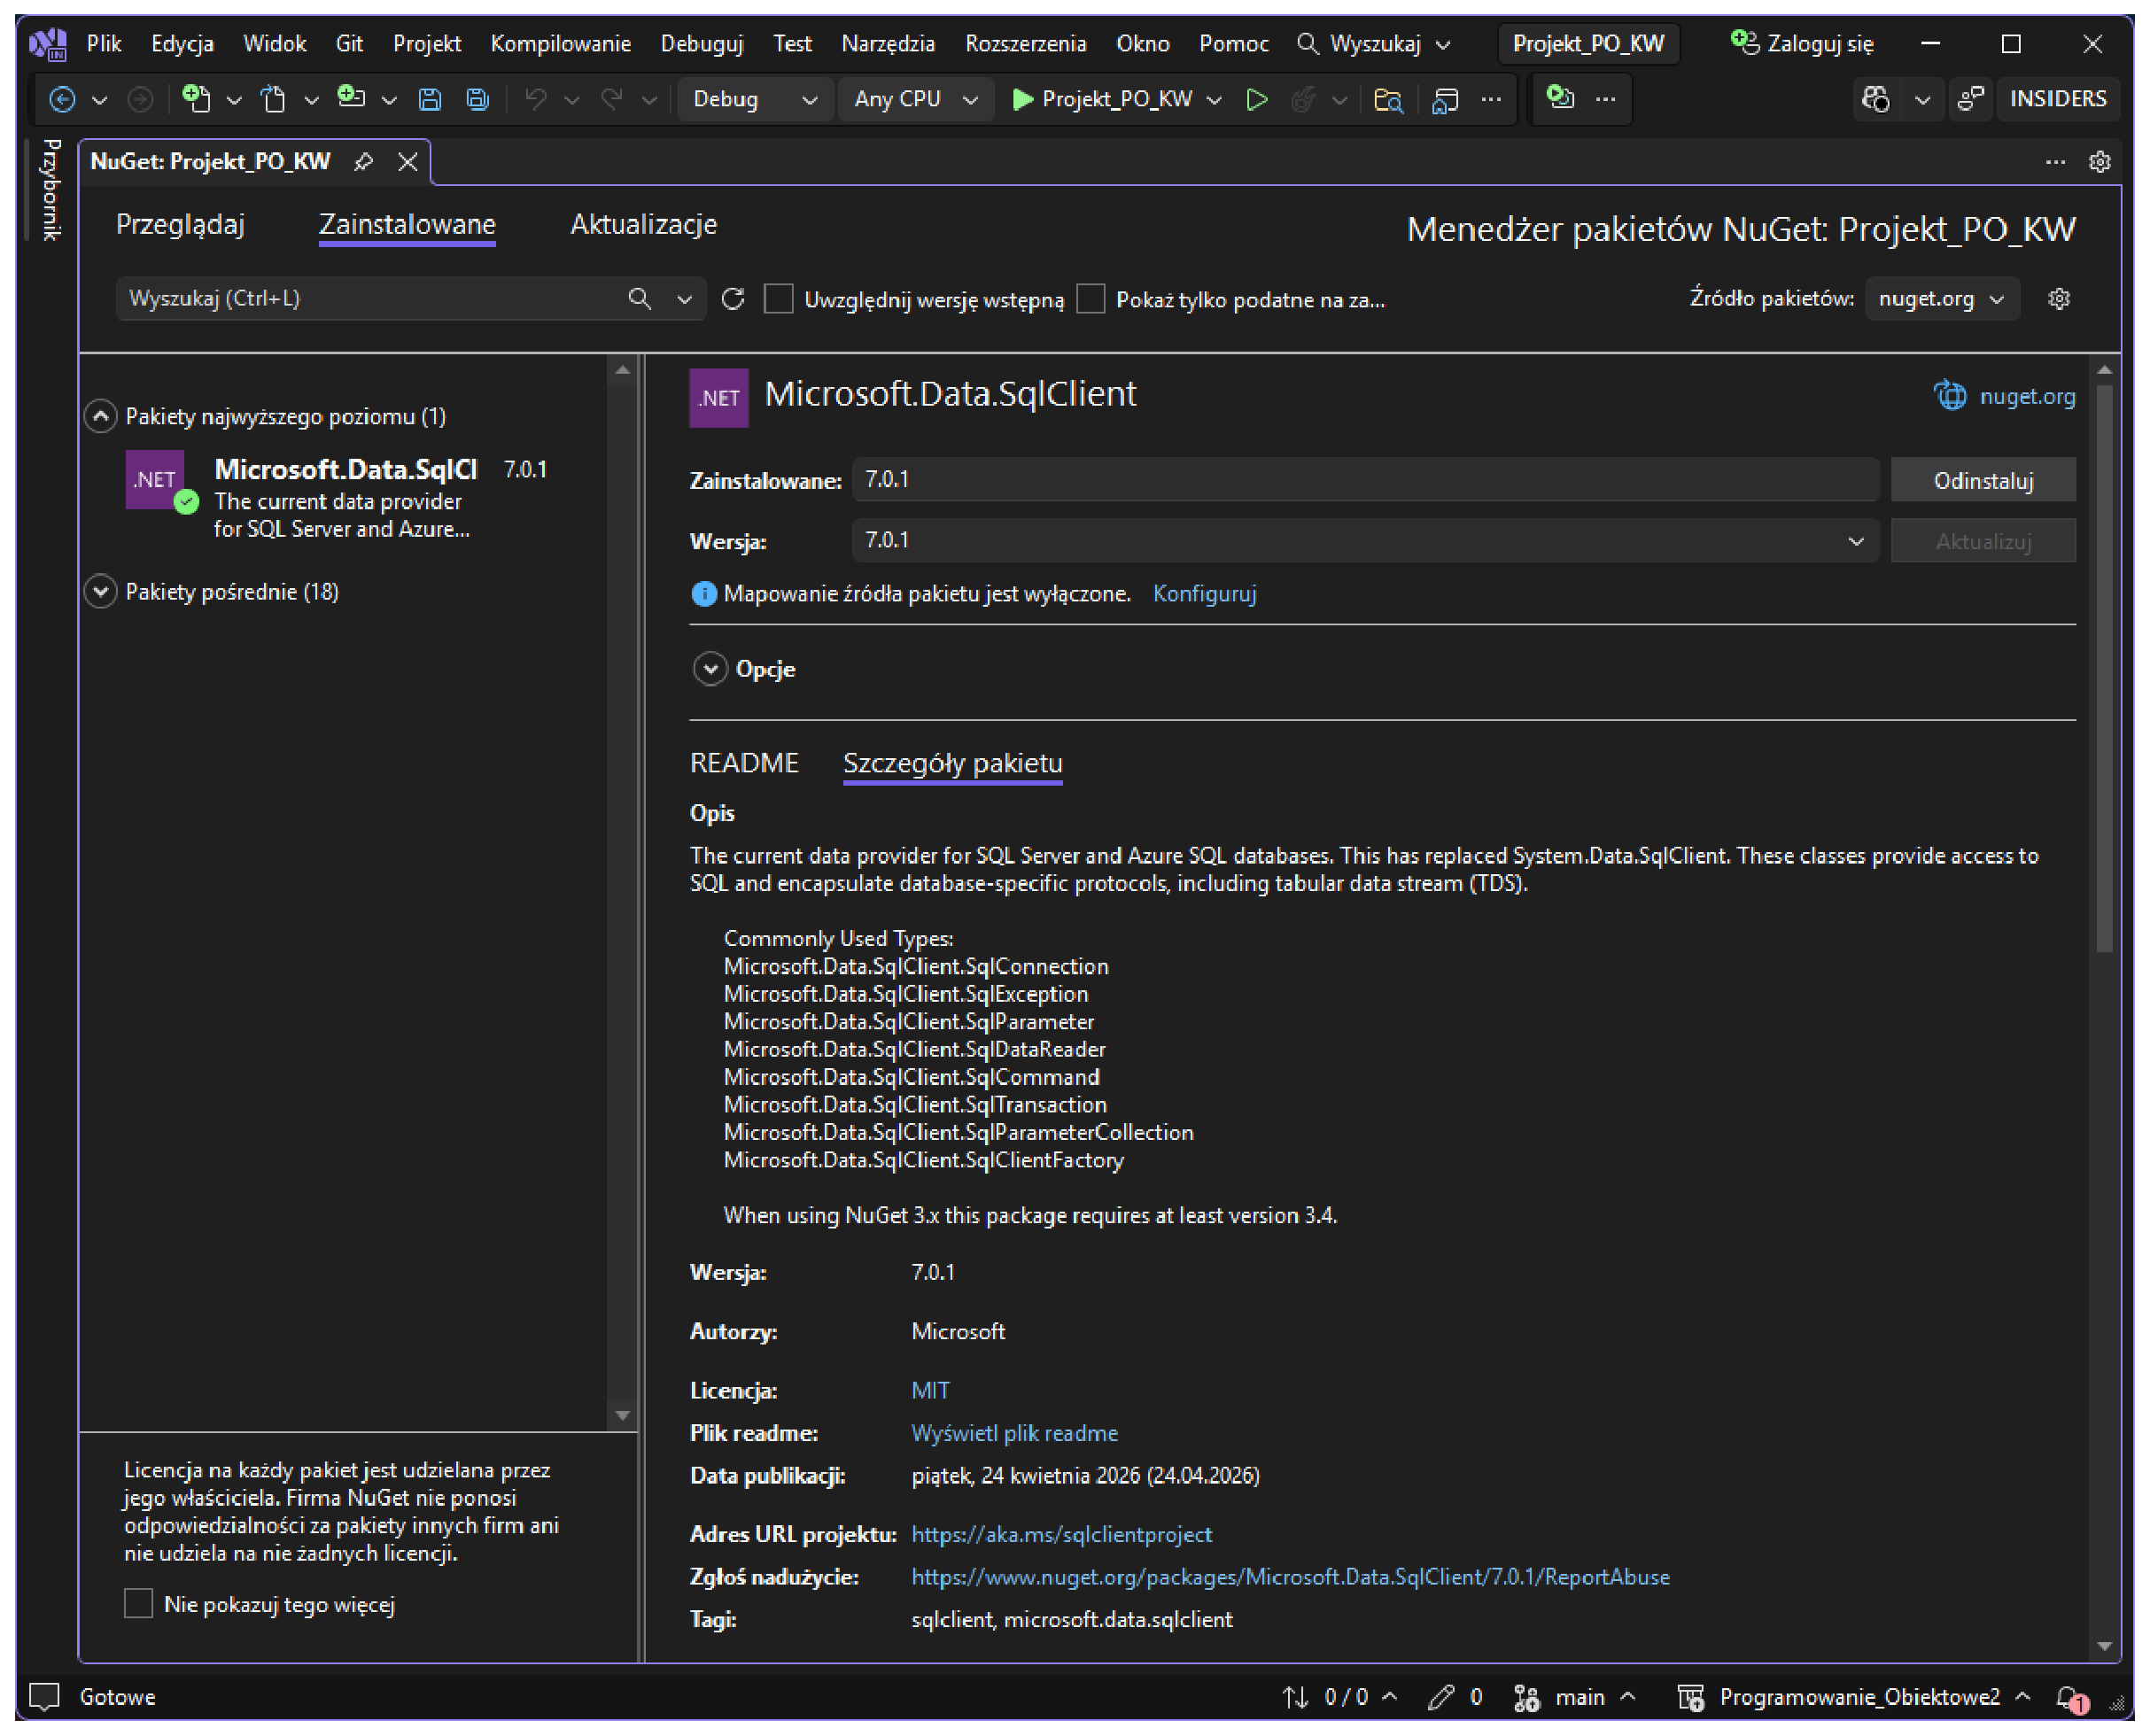
\includegraphics[width=\linewidth]{figures/fig_001.eps}
\caption{Sterownik Microsoft.Data.SqlClient (Menadżer pakietów NuGet).\label{fig1}}
\end{figure}

Baza danych składa się z ośmiu tabel: 
Uzytkownik, Pupil, Weterynarz, Zabieg, 
Rezerwacja, Dostepnosc oraz tabel łączących 
Uzytkownik\_Pupil i Weterynarz\_Zabieg. 
Tabela Uzytkownik oraz Pupil połączone są relacją 
wiele do wielu za pomocą tabeli łączącej Uzytkownik\_Pupil, 
tzn. jeden użytkownik może posiadać wiele pupili i jeden pupil może 
mieć wielu właścicieli. Tabela Weterynarz oraz Zabieg
połączone są relacją wiele do wielu za pomocą tabeli 
Weterynarz\_Zabieg, co oznacza, że jeden weterynarz może 
wykonywać wiele zabiegów, a jeden zabieg może być wykonywany przez 
wielu weterynarzy. Tabela Dostepnosc powiązana jest z tabelą 
Weterynarz relacją jeden do wielu i przechowuje informacje 
o godzinach pracy weterynarza w poszczególnych dniach tygodnia. 
Tabela Rezerwacja stanowi centralną tabelę systemu i łączy 
w sobie informacje o użytkowniku, pupilu, weterynarzu oraz zabiegu, 
przechowując datę, godzinę oraz aktualny status wizyty.

\begin{table}[H]
\centering
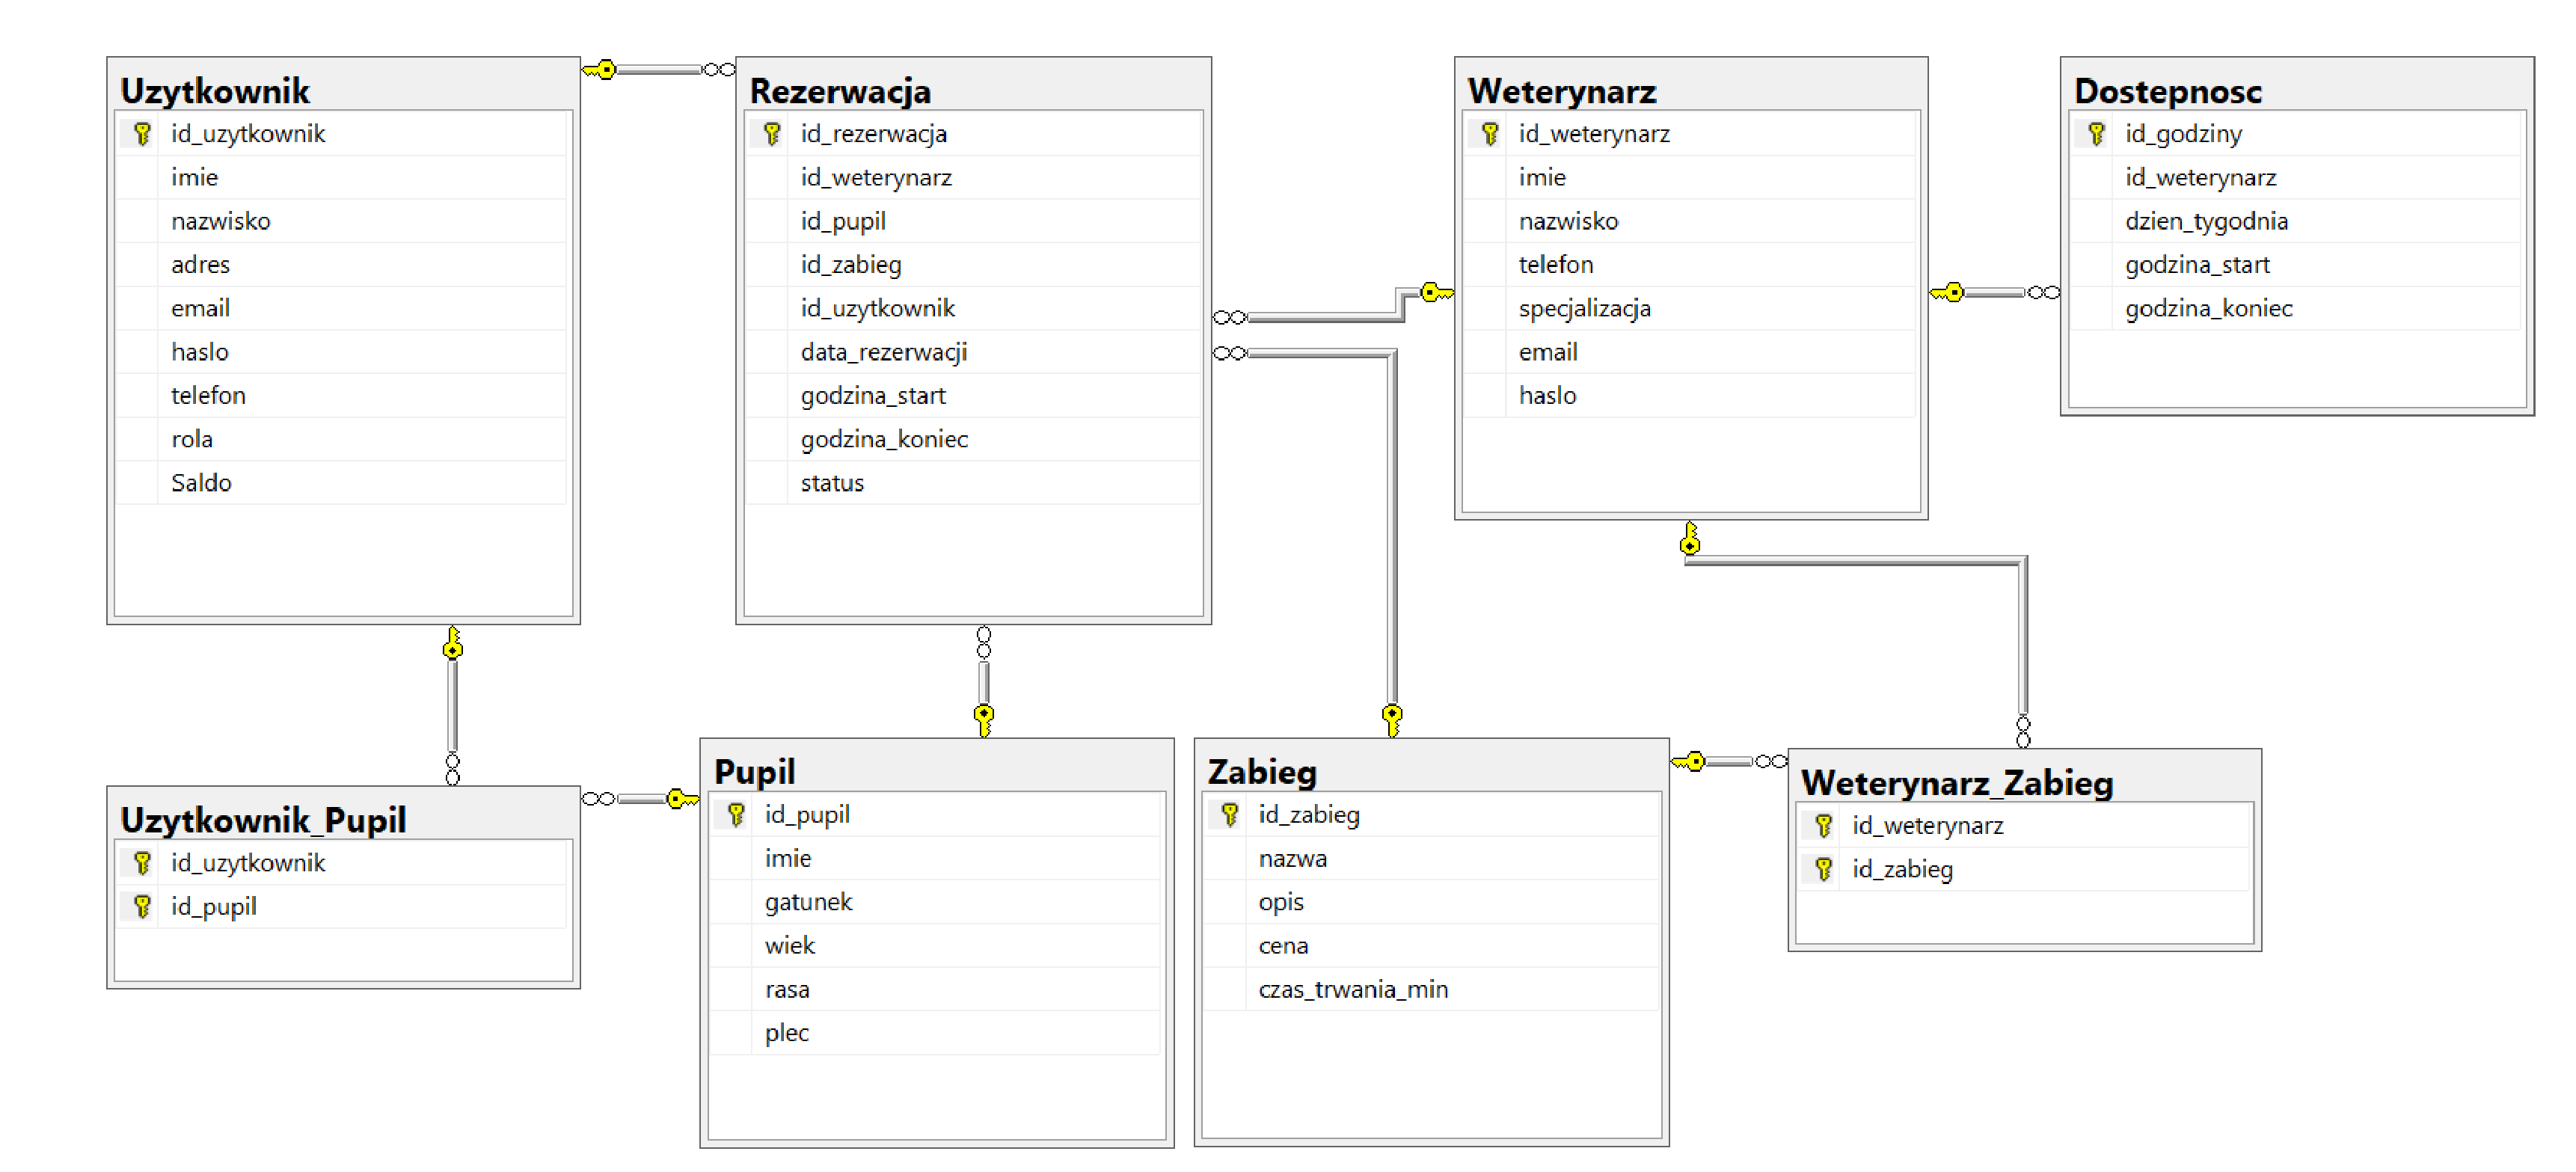
\includegraphics[width=1.15\linewidth]{figures/fig_002.eps}
\caption{Diagram ERD projektowanej aplikacji.\label{fig2}}
\end{table}

\subsection{Normalizacja bazy oraz Integralność danych}

\textbf{Normalizacja bazy danych}

Baza danych została zaprojektowana zgodnie z trzecią postacią normalną (3NF). 
Każda tabela zawiera tylko atrybuty bezpośrednio zależne od klucza głównego, eliminując redundancję 
danych. Relacje wiele do wielu (Uzytkownik-Pupil oraz WeterynarzZabieg) zostały 
rozwiązane przy użyciu dedykowanych tabel łączących.

\textbf{Integralność danych}

Integralność danych w bazie zapewniana jest przez następujące mechanizmy:
\begin{itemize}
\item \textbf{Klucze główne} - każda tabela posiada unikalny identyfikator typu INT IDENTITY, automatycznie 
inkrementowany przez SQL Server,
\item \textbf{Klucze obce} - relacje między tabelami są wymuszane przez ograniczenia FOREIGN KEY, uniemożliwiające 
dodanie rekordów z nieistniejącymi odwołaniami,
\item \textbf{Ograniczenia CHECK} - kolumny gatunek (Pies/Kot), plec (Samiec/Samica), rola (Uzytkownik/Administrator)
oraz status (Zarezerwowany/Anulowany/Zrealizowany) posiadają ograniczenia dopuszczalnych wartości,
\item \textbf{Unikalność} - kolumna email w tabeli Uzytkownik posiada ograniczenie UNIQUE, uniemożliwiające 
rejestrację dwóch kont na ten sam adres e-mail,
\item \textbf{Walidacja po stronie aplikacji} - dodatkowa weryfikacja danych wejściowych realizowana jest w
kodzie C\# przed wykonaniem zapytań do bazy danych, co stanowi drugą warstwę ochrony przed nieprawidłowymi danymi.
\end{itemize}

\section{Struktura klas}

Projekt podzielony jest na cztery warstwy: Models (klasy odwzorowujące tabele bazy danych), 
Repositories (klasy odpowiedzialne za komunikację z bazą danych 
poprzez ADO.NET), Views (okna WPF) oraz 
Helpers (klasy pomocnicze tzn. SessionHelper i DialogHelper). 
Klasa Database odpowiada za nawiązanie 
połączenia z bazą danych SQL Server.

\begin{figure}[H]
\centering
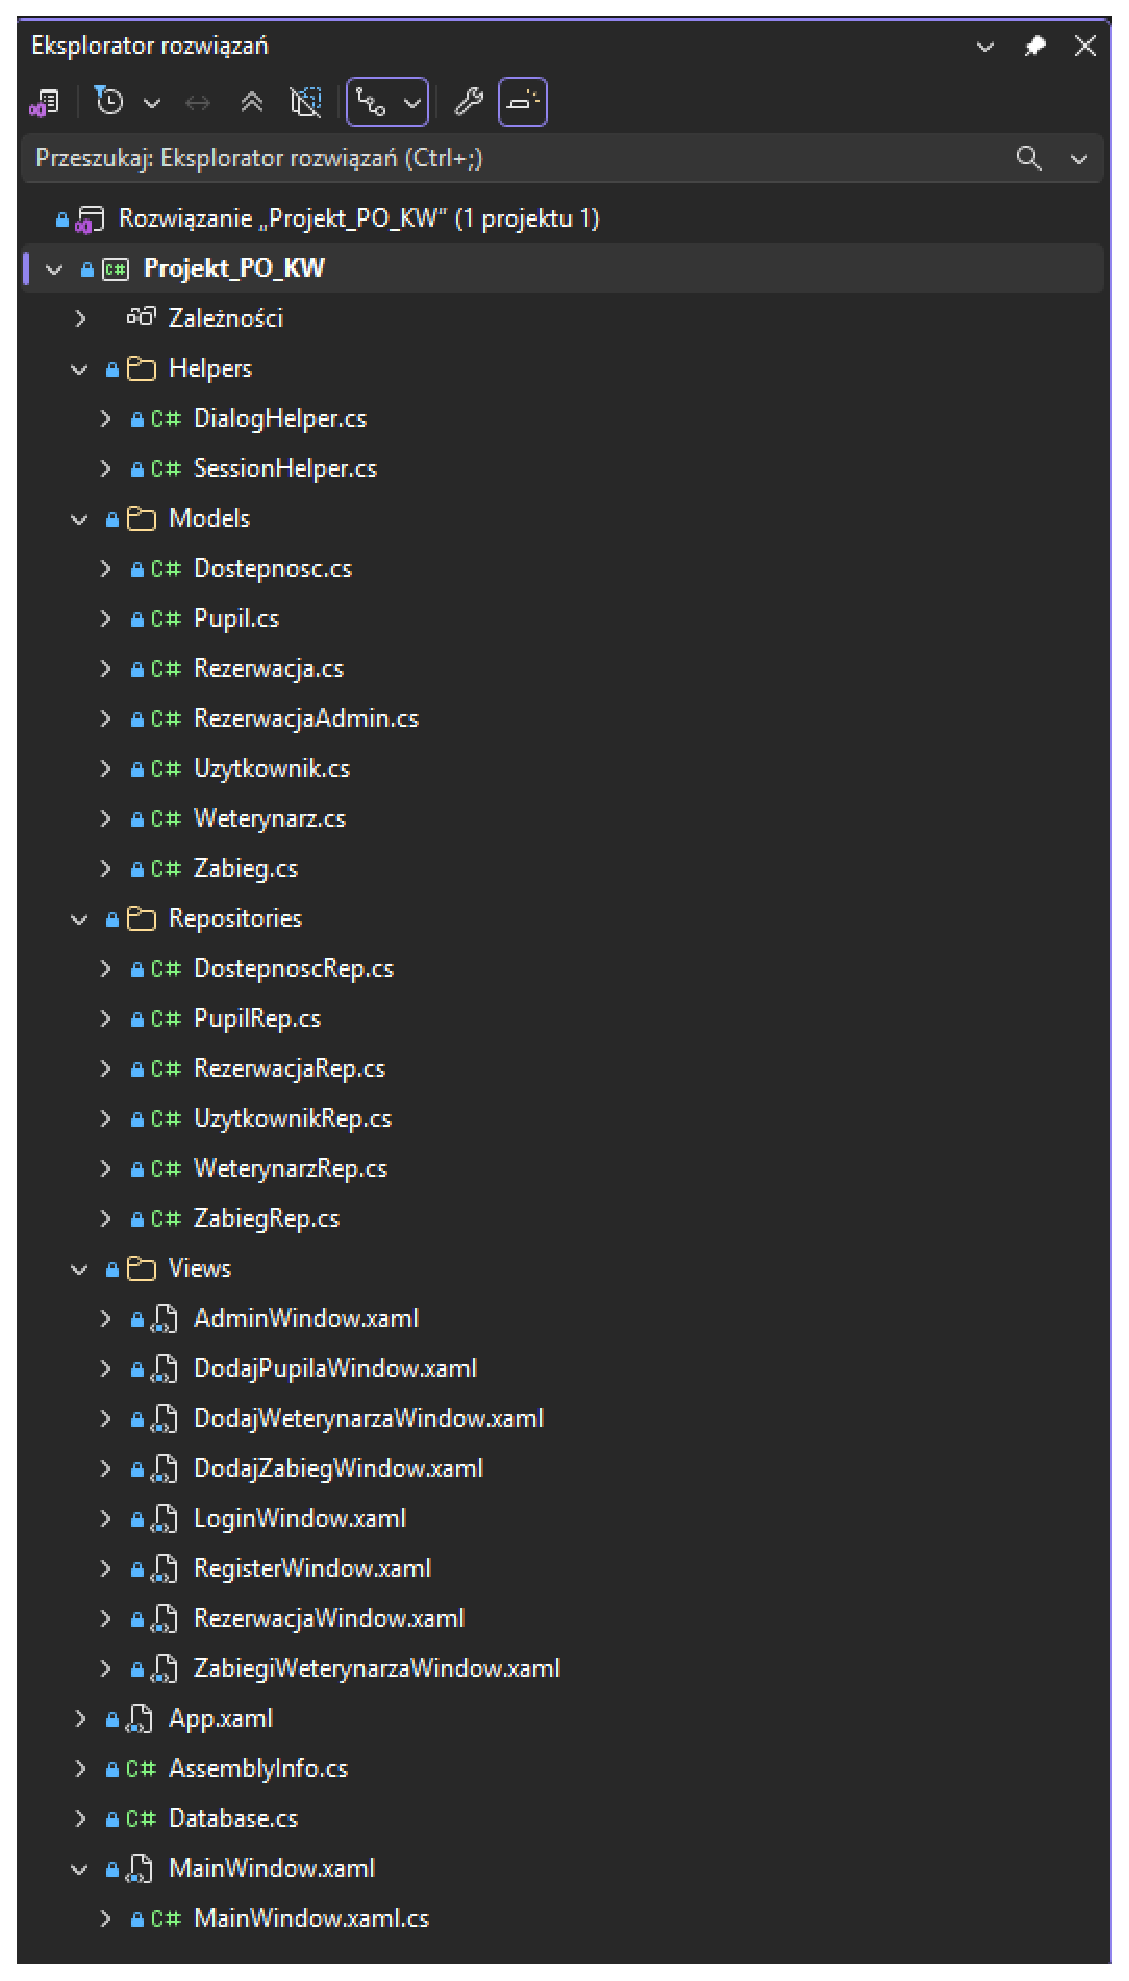
\includegraphics[width=0.9\linewidth]{figures/fig_003.eps}
\caption{Struktura klas w projekcie.\label{fig3}}
\end{figure}

\section{Najważniejsze metody}

\subsection{Logowanie}

Metoda Zaloguj\_sie pobiera wartości z pól formularza: adres e-mail oraz hasło. 
Następnie sprawdza, czy oba pola zostały uzupełnione, jeśli nie to wyświetlany jest komunikat błędu. Jeżeli pola są wypełnione, wywoływana 
jest metoda GetUser z repozytorium UzytkownikRep, która wykonuje zapytanie SQL do bazy danych i zwraca obiekt użytkownika 
na podstawie podanego adresu e-mail oraz hasła. Jeśli użytkownik nie zostanie znaleziony w bazie danych, wyświetlany jest komunikat o 
nieprawidłowych danych logowania. W przypadku pomyślnego uwierzytelnienia dane zalogowanego użytkownika zapisywane są w klasie
SessionHelper, która przechowuje je przez cały czas działania aplikacji. Następnie sprawdzana jest rola przypisana do konta, jeśli jest 
to administrator, otwierany jest panel administratora AdminWindow, w przeciwnym razie otwierany jest panel użytkownika w tym wypadku MainWindow. 
Okno logowania zostaje zamknięte. W przypadku błędu połączenia z bazą danych wyświetlany jest komunikat z informacją o przyczynie błędu.

\lstinputlisting[caption=Metoda logowania wraz z SessionHelper oraz metodą z zapytaniem SQL, label=logowanie]{src/Task1.cs}

\subsection{Zmiana hasła - panel użytkownika}

Metoda Zmiana\_hasla pobiera dane zalogowanego użytkownika z klasy SessionHelper. 
Następnie odczytuje wartości z trzech pól formularza tzn. obecne hasło, nowe hasło oraz potwierdzenie hasła. 
Sprawdza, czy wszystkie pola zostały uzupełnione jeśli nie, wyświetlany jest komunikat błędu. Następnie weryfikuje, 
czy podane obecne hasło zgadza się z hasłem przechowywanym w sesji jeśli nie, wyświetlany jest komunikat o nieprawidłowym haśle.
Kolejnym krokiem jest sprawdzenie, czy nowe hasło jest identyczne z polem potwierdzającym oraz czy jego długość wynosi co najmniej 6 znaków.
Przed wykonaniem zmiany użytkownik proszony jest o potwierdzenie operacji w oknie dialogowym. Następnie wywoływana jest metoda Zmiana\_hasla 
z repozytorium UzytkownikRep, która wykonuje 
zapytanie UPDATE aktualizujące hasło w bazie danych na podstawie identyfikatora użytkownika. Po pomyślnym wykonaniu operacji pola formularza zostają 
wyczyszczone, a użytkownik otrzymuje komunikat o sukcesie. W przypadku błędu połączenia z bazą danych wyświetlany 
jest komunikat z informacją o przyczynie błędu.

\lstinputlisting[caption=Metoda zmiany hasła wraz z metodą zapytania SQL, label=zmiana hasla]{src/Task2.cs}

\subsection{Zmiana panelu wyświetlania - panel użytkownika}

Metoda Nav\_Click odpowiada za nawigację między sekcjami panelu użytkownika. Na początku wszystkie 
panele tzn. PanelMojeKonto, PanelMojePupile, PanelMojeWizyty oraz PanelDoladujSrodki są ukrywane poprzez 
ustawienie właściwości Visibility na Collapsed, a znaczniki aktywności wszystkich przycisków nawigacyjnych są zerowane. 
Następnie kliknięty przycisk zostaje oznaczony jako aktywny poprzez ustawienie jego właściwości Tag na wartość active. W zależności od 
tego, który przycisk został kliknięty, wyświetlany jest odpowiedni panel. 
W przypadku sekcji Moje pupile dodatkowo wywoływana jest metoda WczytajPupile, która pobiera listę pupili zalogowanego 
użytkownika z bazy danych. Analogicznie w przypadku sekcji Moje wizyty wywoływana jest metoda WczytajWizyty, która pobiera 
historię rezerwacji użytkownika.

\lstinputlisting[caption=Metoda nawigacji do zmiany panelu wyświetlania, label=zmiana panelu wyświetlania]{src/Task3.cs}

\subsection{Wpłata środków - panel użytkownika}

Metoda WplacSrodki\_Click umożliwia użytkownikowi doładowanie salda konta. Pobiera wartość wpisaną przez użytkownika 
w polu tekstowym i próbuje przekonwertować ją na liczbę całkowitą przy użyciu metody int.TryParse. 
Jeśli podana wartość nie jest liczbą całkowitą lub jest mniejsza bądź równa zero, wyświetlany jest komunikat błędu. W przypadku 
poprawnych danych użytkownik proszony jest o potwierdzenie operacji w oknie dialogowym. Po zatwierdzeniu wywoływana jest 
metoda DoladujSaldo z repozytorium UzytkownikRep, która wykonuje zapytanie UPDATE zwiększające saldo 
użytkownika w bazie danych o podaną kwotę. Jednocześnie saldo aktualizowane jest w obiekcie przechowywanym w SessionHelper 
oraz odświeżana jest etykieta wyświetlająca aktualne saldo w interfejsie użytkownika. Pole tekstowe zostaje wyczyszczone, a użytkownik 
otrzymuje komunikat o pomyślnym wykonaniu wpłaty. W przypadku błędu połączenia z bazą danych wyświetlany jest 
komunikat z informacją o przyczynie błędu.

\lstinputlisting[caption=Metoda wpłaty środków wraz z metodą zapytania SQL, label=wpłata środków]{src/Task4.cs}

\subsection{Rezerwacja zabiegu - panel użytkownika}

Metoda WybierzZabieg obsługuje wybór zabiegu przez użytkownika w pierwszym kroku rezerwacji. 
Na początku iteruje po wszystkich elementach listy zabiegów i resetuje kolor obramowania każdego z nich do 
domyślnego koloru szarego, aby usunąć poprzednie zaznaczenie. Następnie pobiera kliknięty element jako obiekt Border i zmienia 
kolor jego obramowania na różowy, sygnalizując aktywny wybór. Wybrany zabieg zostaje zapisany w polu \_wybranyZabieg
jako obiekt typu Zabieg, pobierany z kontekstu danych klikniętego elementu.

\lstinputlisting[caption=Metoda wyboru zabiegu oraz wyboru weterynarza, label=Rezerwacja zabiegu (1-3)]{src/Task5.cs}

Metoda Dalej\_Click obsługuje nawigację między trzema krokami procesu rezerwacji wizyty. W pierwszym kroku sprawdza, czy 
użytkownik wybrał pupila z listy rozwijanej oraz czy zaznaczył zabieg jeśli nie, wyświetlany jest odpowiedni komunikat błędu. 
Następnie weryfikuje, czy saldo konta użytkownika jest wystarczające do pokrycia kosztu wybranego zabiegu. Jeśli środki są niewystarczające,
wyświetlany jest komunikat informujący o aktualnym saldzie oraz koszcie zabiegu. W przypadku poprawnej walidacji pobierana jest lista weterynarzy 
wykonujących wybrany zabieg przy użyciu metody GetByZabieg z repozytorium WeterynarzRep, która wykonuje zapytanie SELECT z 
połączeniem tabel Weterynarz i Weterynarz\_Zabieg. W drugim kroku sprawdzane jest, czy 
użytkownik wybrał weterynarza jeśli tak, wywoływana jest metoda WygenerujKalendarz i interfejs przełącza się na trzeci krok, a przycisk Dalej
zmienia treść na Zarezerwuj. W trzecim a zarazem ostatnimkroku sprawdzane jest, czy użytkownik wybrał termin jeśli tak, wywoływana jest metoda ZapiszRezerwacje.

\lstinputlisting[caption=Metoda do rezerwacji (zachowania ciągłąści między etapami) wraz z metodą zapytania SQL, label=Rezerwacja zabiegu (2-3)]{src/Task6.cs}

Metoda WygenerujKalendarz odpowiada za dynamiczne generowanie tygodniowego widoku kalendarza dostępności wybranego 
weterynarza. Na początku czyszczone są wszystkie elementy siatki kalendarza. Następnie pobierana jest dostępność weterynarza z 
bazy danych przy użyciu metody GetByWeterynarz z repozytorium DostepnoscRep, która wykonuje 
zapytanie SELECT zwracające godziny pracy weterynarza w poszczególnych dniach tygodnia. Na podstawie pobranych danych 
generowana jest lista dni tygodnia od dnia dzisiejszego, dla których weterynarz ma zdefiniowane godziny pracy. Dla każdego dnia dodawana 
jest kolumna do siatki kalendarza z nagłówkiem zawierającym nazwę dnia i datę. Następnie pobierane są istniejące rezerwacje weterynarza z 
bazy danych. Dla każdej godziny od 8:00 do 16:00 oraz dla każdego dostępnego dnia generowany jest przycisk, którego stan zależy od trzech 
warunków: czy dany slot mieści się w godzinach pracy weterynarza, czy godzina zakończenia zabiegu nie przekracza końca jego pracy oraz czy 
w danym terminie nie istnieje już inna rezerwacja. Przyciski oznaczone są kolorami tzn. zielonym dla wolnych terminów, czerwonym dla zajętych 
oraz szarym dla terminów poza godzinami pracy. Po kliknięciu wolnego slotu poprzednio wybrany termin zostaje zresetowany, a nowo wybrany 
zostaje podświetlony na różowo z etykietą Wybrano. Wybrana data i godzina zapisywane są w odpowiednich polach.

\lstinputlisting[caption=Metoda wyświetląjąca kalendarz wraz z metodą zapytania SQL, label=Rezerwacja zabiegu (3-3)]{src/Task7.cs}

\subsection{Lista użytkowników - panel administratora}

Metoda WczytajUzytkownikow pobiera listę wszystkich zarejestrowanych użytkowników z bazy danych przy użyciu metody 
GetAllUzytkownicy z repozytorium UzytkownikRep i przypisuje ją jako źródło danych do listy użytkowników 
w interfejsie. Metoda GetAllUzytkownicy wykonuje zapytanie SELECT pobierające wszystkich użytkowników z 
rolą Uzytkownik, posortowanych według nazwiska.

Metoda UsunUzytkownika\_Click obsługuje usunięcie użytkownika przez administratora. 
Pobiera identyfikator użytkownika z właściwości Tag klikniętego przycisku i wyświetla okno 
dialogowe z prośbą o potwierdzenie operacji, informując że usunięcie użytkownika spowoduje również usunięcie 
jego pupili i rezerwacji. Po potwierdzeniu wywoływana jest metoda UsunUzytkownika z 
repozytorium UzytkownikRep i lista użytkowników jest odświeżana. Metoda UsunUzytkownika
wykonuje operację usunięcia w kilku krokach: najpierw usuwa wszystkie rezerwacje użytkownika, następnie pobiera listę 
jego pupili, usuwa powiązania użytkownika z pupilami z tabeli Uzytkownik\_Pupil, a następnie 
dla każdego pupila sprawdza, czy nie posiada już innych właścicieli jeśli nie, pupil zostaje trwale usunięty z tabeli 
Pupil. Na końcu usuwany jest sam rekord użytkownika z tabeli Uzytkownik.

\lstinputlisting[caption=Metody usuwania i wczytywania użytkowników wraz z metodą zapytania SQL, label=lista użytkowników]{src/Task8.cs}

\subsection{Dodawanie weterynarza - panel administratora}

Metoda DodajWeterynarza\_Click obsługuje dodawanie nowego weterynarza przez administratora. Pobiera wartości ze wszystkich 
pól formularza i sprawdza, czy wymagane pola (imię, nazwisko, email oraz hasło) zostały uzupełnione jeśli nie, wyświetlany jest 
komunikat błędu. W przypadku poprawnej walidacji wywoływana jest metoda Dodaj z repozytorium WeterynarzRep, 
która wykonuje zapytanie INSERT dodające nowego weterynarza do tabeli Weterynarz w bazie danych. Następnie 
pobierany jest identyfikator nowo dodanego weterynarza przy użyciu metody GetIdByEmail. Dla każdego dnia tygodnia od 
poniedziałku do piątku wywoływana jest metoda pomocnicza ZapiszDostepnosc, która sprawdza, czy pola godzin zostały 
uzupełnione oraz czy godzina rozpoczęcia jest wcześniejsza niż godzina zakończenia jeśli warunki są spełnione, wywoływana 
jest metoda Dodaj z repozytorium DostepnoscRep, która wykonuje zapytanie INSERT zapisujące godziny 
pracy weterynarza w danym dniu tygodnia do tabeli Dostepnosc. Jeśli pola godzin dla danego dnia są puste, wpis dla 
tego dnia nie jest tworzony, co oznacza że weterynarz nie pracuje w tym dniu.

\lstinputlisting[caption=Metoda dodawania weterynarza wraz z metodami zapytań SQL, label=dodawanie weterynarza]{src/Task9.cs}

\subsection{Dodawanie zabiegu - panel administratora}

Metoda Dodaj\_Click w oknie DodajZabiegWindow obsługuje dodawanie 
nowego zabiegu przez administratora. Pobiera wartości z trzech pól formularza: nazwę zabiegu, czas trwania oraz cenę. 
Sprawdza, czy wszystkie pola zostały uzupełnione jeśli nie, wyświetlany jest komunikat błędu. Następnie weryfikuje, 
czy podany czas trwania jest poprawną dodatnią liczbą całkowitą przy użyciu metody int.TryParse, oraz czy cena 
jest poprawną nieujemną liczbą dziesiętną przy użyciu metody decimal.TryParse. W przypadku poprawnej walidacji 
wywoływana jest metoda Dodaj z repozytorium ZabiegRep, która wykonuje zapytanie INSERT dodające nowy 
zabieg do tabeli Zabieg w bazie danych. Pole opis jest opcjonalne jeśli nie zostało uzupełnione, do bazy zapisywana 
jest wartość NULL. 

Natomiast metoda UsunZabieg\_Click obsługuje usunięcie zabiegu. Pobiera identyfikator zabiegu z właściwości Tag
klikniętego przycisku i wyświetla okno dialogowe z prośbą o potwierdzenie operacji, informując że usunięcie zabiegu spowoduje również usunięcie 
powiązanych rezerwacji. Po potwierdzeniu wywoływana jest metoda Usun z repozytorium ZabiegRep, która wykonuje operację usunięcia 
w trzech krokach: najpierw usuwa wszystkie rezerwacje powiązane z danym zabiegiem z tabeli Rezerwacja, następnie usuwa powiązania z 
weterynarzami z tabeli Weterynarz\_Zabieg, a na końcu usuwa sam rekord zabiegu z tabeli Zabieg. 
Po pomyślnym usunięciu lista zabiegów jest odświeżana.

\lstinputlisting[caption=Metody dodawania i usuwania zabiegów wraz z metodami zapytań SQL, label=dodawanie zabiegu]{src/Task10.cs}

\subsection{Operacje na zabiegach - panel administratora}

Metoda WczytajRezerwacje pobiera wszystkie rezerwacje z bazy danych przy użyciu metody GetAllAdmin z repozytorium RezerwacjaRep, 
która wykonuje zapytanie SELECT z czterokrotnym połączeniem tabel Weterynarz, Pupil, Zabieg, Uzytkownik w 
celu pobrania pełnych informacji o każdej rezerwacji, takich jak imię i nazwisko weterynarza, imię pupila, nazwa zabiegu oraz imię i nazwisko właściciela.
Wyniki są sortowane malejąco według daty rezerwacji. Pobrana lista zapisywana jest w polu \_wszystkieRezerwacje, a 
następnie wywoływana jest metoda ZastosujFiltry.

Metoda ZastosujFiltry filtruje listę wszystkich rezerwacji na podstawie trzech kryteriów: wybranej daty, wybranego weterynarza oraz wybranego statusu. 
Filtrowanie odbywa się sekwencyjnie tzn. każdy aktywny filtr zawęża zbiór wyników. Aby uniknąć wywoływania filtrowania podczas inicjalizacji kontrolek, metoda 
sprawdza flagę \_inicjalizacja. Metoda WyczyscFiltry\_Click resetuje wszystkie filtry do wartości domyślnych i ponownie wywołuje ZastosujFiltry.

Metoda StatusRezerwacji\_Changed obsługuje zmianę statusu rezerwacji bezpośrednio z poziomu listy. 
Pobiera identyfikator rezerwacji z właściwości Tag listy rozwijanej oraz nową wartość statusu z wybranego elementu. 
Następnie wywołuje metodę ZmienStatus z repozytorium RezerwacjaRep, która wykonuje zapytanie UPDATE
aktualizujące status rezerwacji w bazie danych.

Metoda AktualizujPrzeterminowane wywoływana jest automatycznie przy każdym uruchomieniu aplikacji w klasie App.xaml.cs. 
Wykonuje zapytanie UPDATE zmieniające status wszystkich rezerwacji o statusie Zarezerwowany, których godzina 
zakończenia już minęła, na status Zrealizowany. Dzięki temu system automatycznie aktualizuje historię wizyt.

\lstinputlisting[caption=Metoda aktualizacji statusów oraz metody związane z zabiegami wraz z metodami zapytań SQL, label=lista zabiegów]{src/Task11.cs}

\section{Wymagania sprzętowe i narzędzia}

\begin{itemize}
\item \textbf{Procesor:} minimum 2-rdzeniowy, 2.0 GHz lub szybszy.
\item \textbf{Pamięć RAM:} minimum 8 GB.
\item \textbf{System operacyjny:} Windows 10 (64-bit) lub nowszy.
\item \textbf{.NET:} wersja 10.0 lub nowsza.
\item \textbf{Microsoft SQL Server:} wersja 2025 (wersja używana w projekcie).
\item \textbf{Visual Studio Insiders:} wersja 2026 (wersja używana w projekcie).
\item \textbf{Sterownik ADO.NET:} Microsoft.Data.SqlClient w wersji 7.0.1 
(instalowany przez NuGet).
\end{itemize}

\textbf{Narzędzia wykorzystane w projekcie}

\begin{itemize}
\item \textbf{Visual Studio Insiders 2026} - środowisko programistyczne do tworzenia aplikacji w języku C\#,
\item \textbf{Git} - system kontroli wersji,
\item \textbf{WPF (Windows Presentation Foundation)} - technologia do tworzenia graficznego interfejsu użytkownika,
\item \textbf{Microsoft SQL Server 2025} - system zarządzania relacyjną bazą danych,
\item \textbf{SQL Server Management Studio (SSMS)} - narzędzie do zarządzania bazą danych SQL Server,
\item \textbf{Microsoft.Data.SqlClient 7.0.1} - sterownik ADO.NET do komunikacji z bazą danych SQL Server,
\item \textbf{Strona online-convert.com} - strona wykorzystana do konwersji grafik do formatu EPS.
\end{itemize}